\documentclass{article}

\usepackage{amsmath}
\usepackage{graphicx}
\usepackage{multicol}
\usepackage{color}
\usepackage{comment}
\usepackage{tikz}
\usetikzlibrary{shapes.geometric,arrows,fit}
\oddsidemargin 0cm
\evensidemargin 0cm

\textwidth 16.5cm
\topmargin -2.0cm
\parindent 0cm
\textheight 24cm
\parskip 0.5cm

\usepackage{fancyhdr}
\pagestyle{fancy}
\fancyhf{}
%\fancyhead[L]{AOSS Reference Sheet}
%\fancyhead[CH]{test}
\fancyfoot[C]{Page \thepage}

\begin{document}
{\Huge \textbf{BlobMetrics: an analysis framework for StitchBlobs outputs}}
\tableofcontents

\pagebreak

\section{Minimum software and data requirements}
\begin{itemize}
\item R software (\texttt{https://www.r-project.org/}) and the following libraries:
\begin{itemize}
\item \texttt{abind} (\texttt{readnetcdf.R})
\item \texttt{akima} (\texttt{readnetcdf.R}, \texttt{intercomparison.R}, \texttt{pearsonrmse.R})
\item \texttt{argparse} (\texttt{stitch\_metric\_framework.R})
\item \texttt{ggplot2} (\texttt{generateReport.R})
\item \texttt{gtable} (\texttt{generateReport.R})
\item \texttt{grid} (\texttt{generateReport.R})
\item \texttt{knitr} (\texttt{generateReport.R})
\item \texttt{markdown} (\texttt{generateReport.R})
\item \texttt{ncdf4} (\texttt{readnetcdf.R)}
\item \texttt{ncdf4.helpers} (\texttt{readnetcdf.R})
\item \texttt{PCICt} (\texttt{readnetcdf.R})
\item \texttt{reshape2} (\texttt{intercomparison.R},\texttt{pearsonrmse.R})
\item \texttt{rmarkdown} (\texttt{generateReport.R})
\item \texttt{RNetCDF} (\texttt{readnetcdf.R})
\end{itemize}
\item StitchBlobs output (in the form of NetCDF files)
\item BlobStats output (in the form of text files)
\end{itemize}



\section{Usage}
\subsection{Command line usage}
The main control framework is run from the command line, with the following syntax:
\begin{verbatim}
Rscript --vanilla stitch_metric_framework.R [flags]
\end{verbatim}

In order to view all possible options, run the above command with the \texttt{-h} or \texttt{--help} flag:
\begin{verbatim}
Rscript --vanilla stitch_metric_framework.R -h
\end{verbatim}

which will print out the list of available flags and exit. These flags will be explained further in subsequent sections.

\subsubsection{Namelists}
Each utility must be used in conjunction with a namelist file, which will provide all of the necessary variables that are not specified in the command line. Example namelists are included in the directory with the R function source files.

The \texttt{-nl} or \texttt{--namelist} flag specifies the master namelist, which contains the necessary variables for all of the framework utilities. However, each utility can be provided with a separate namelist file if desired (flags specified in subsequent sections), which will override inputs from the master namelist.

For example, 

\begin{verbatim}
Rscript --vanilla stitch_metric_framework.R  -nl namelist_master.R -rf
-mt -st -nlst namelist_summarize.R
\end{verbatim}

will use \texttt{namelist\_master.R} for the \texttt{--readfiles} and \texttt{--mergetable} utilities but \texttt{namelist\_summarize.R} for \texttt{--summarize}

%There is an option to generate a master namelist file for all of the various analysis operations, using an initial list of variables. A template for this initial list is generated by running the command
%
%\begin{verbatim}
%Rscript --vanilla gen_blank_setupfile.R
%\end{verbatim}
%
%which returns the file \texttt{blank\_setupfile.R} with all of the required variables. Fill in the desired values and then save the modified file with your desired name (example, \texttt{setup\_reanalysis.R})
%
%Then, run the command
%
%\begin{verbatim}
%Rscript --vanilla stitch_metric_framework.R -gn -sl [name of setup list]
%\end{verbatim}
%
%which will return a master namelist file with all of the variables filled in. Examples of \texttt{blank\_setupfile.R}, a modified version with all of the variables filled in (\texttt{setup\_full.R}), and the resultant master namelist (\texttt{DJF\_NP\_namelist\_master\_test.R}) can be found in the \texttt{STITCH\_METRICS} directory.

\subsection{Example workflow: running BlobMetrics for the first time}

After downloading the repository from Github, navigate to the folder containing all of the R scripts (generally \texttt{tempestextremes/src/blobmetrics}). 
\begin{enumerate}
\item Download the necessary libraries for running the code:
\begin{verbatim}
Rscript --vanilla download_libraries.R
\end{verbatim}

Note that some of the libraries require compiling and installation might fail if the requisite compilers are not available. If a package fails, then the files with the package dependencies (noted next to the package name) will not run. 
\item Prepare all of the necessary input files:
\begin{itemize}
\item a list of files containing all of the BlobStats output using StitchBlobs input (with full path names)
\item (optional) a list of files containing all of the BlobStats output using DetectBlobs input (with full path names)
\item a list of files containing all of the StitchBlobs output (with full path names)
\end{itemize}
\item Generate the template for creating the master namelist file
\begin{verbatim}
Rscript --vanilla gen_blank_setupfile.R
\end{verbatim}

This will return the file \texttt{blank\_setupfile.R} with all of the required variables (an example of this file can be found in the \texttt{blobmetrics} directory). Fill in the desired values and save the modified file with the desired filename (see example file \texttt{setup\_full.R} in the \texttt{blobmetrics} directory).
\item Generate the master namelist file:
\begin{verbatim}
Rscript --vanilla stitch_metric_framework.R -gn -sl [setup list file]
\end{verbatim}

It will create a new directory (if it doesn't yet exist) with the name specified in the setup file; the master namelist file can be found in this directory. (See example \texttt{text}
\item Run one or more of the desired utilities:
\begin{verbatim}
Rscript --vanilla stitch_metric_framework.R [flags] -nl [namelist]
\end{verbatim}
\end{enumerate}


%Each utility has certain mandatory variables. The \texttt{nrun\_*} variable specifies how many times the utility is to be run; if more than 1, then the variables must be specified as vectors, which have the syntax \texttt{c(VAR1,VAR2,VAR3...)}. For example, to read in data from 4 different datasets using \texttt{--readfiles}:
%
%\begin{verbatim}
%#Location of working directory
%work_dir<-"~/tempestextremes/test/STITCH_METRICS"
%#Location where the input data files are stored
%input_dir<-"~/tempestextremes/test/STITCH_METRICS"
%#Location where the output data files are stored
%output_dir<-"~/tempestextremes/test/STITCH_METRICS"
%
%#This will be run 4 times 
%nrun_rf<-4
%##################################
%###USER-DEFINED###
%#Input file names
%list_files<-c("stitch_list","nostitch_list","merra_list","merra_nolist")
%#output file names
%list_rnames<-c("table_estitch.RData","table_enostitch.RData",
%"table_mstitch.RData","table_mnostitch.RData")
%#Data frame variable names
%list_dfnames<-c("df_estitch","df_enostitch","df_mstitch","df_mnostitch")
%##################################
%
%nhrs<-6
%varname<-c("ERA","ERA","MERRA","MERRA")
%filename_stitchblobs<-""
%filelist_stitchblobs<-paste(input_dir,list_files,sep="/")
%rfn_stitch<-paste(output_dir,list_rnames,sep="/")
%df_stitchname<-list_dfnames
%txt_stitch<-""
%csv_stitch<-""
%\end{verbatim}
%
%Note that some variables, such as \texttt{nhrs} and \texttt{txt\_stitch}, have only one input rather than a vector of 4 values. That value will be used for all runs.
%
%The \texttt{paste} function appends the appropriate directory to the vectors of input and output file names.


%\subsection{Interactive R Usage}
%These various tools can also be utilized in an interactive R session by opening R and loading the various functions from the source R scripts. For example, to read a list of BlobStats files into a single \texttt{data.frame}, type the following commands into R:
%
%\begin{verbatim}
%source("read_stitch.R")
%file_list<-readLines("list_of_blobfiles.txt")
%table_stats<-read_stats_to_table(file_list,6,var="TM90")
%\end{verbatim}
%
%The \texttt{source} command reads in all of the commands from the R script \texttt{read\_stitch.R}, which loads the function \texttt{read\_stats\_to\_table}. This function takes an existing text file (\texttt{list\_of\_blobfiles.txt}) containing a list of BlobStats file names, loads the file names into a vector of strings, and reads all of those files into a data frame that is named \texttt{table\_stats}. \texttt{6} refers to the number of hours per time step in the original data and \texttt{TM90} refers to the block detection algorithm (Tibaldi and Molteni 1990) that was used to produce input files for StitchBlobs. 

\section{BlobMetrics Utilities}

BlobMetrics takes StitchBlobs information in the form of both text files containing per-timestep blob information (min/max lat/lon extent, lat/lon center coordinates, and area) as well as the NetCDF files with the original blobs, turns them into R-compatible datasets, and provides summary information about the blocks in an output report. The framework is outlined in Figure \ref{fig:schematic}.

\begin{figure}
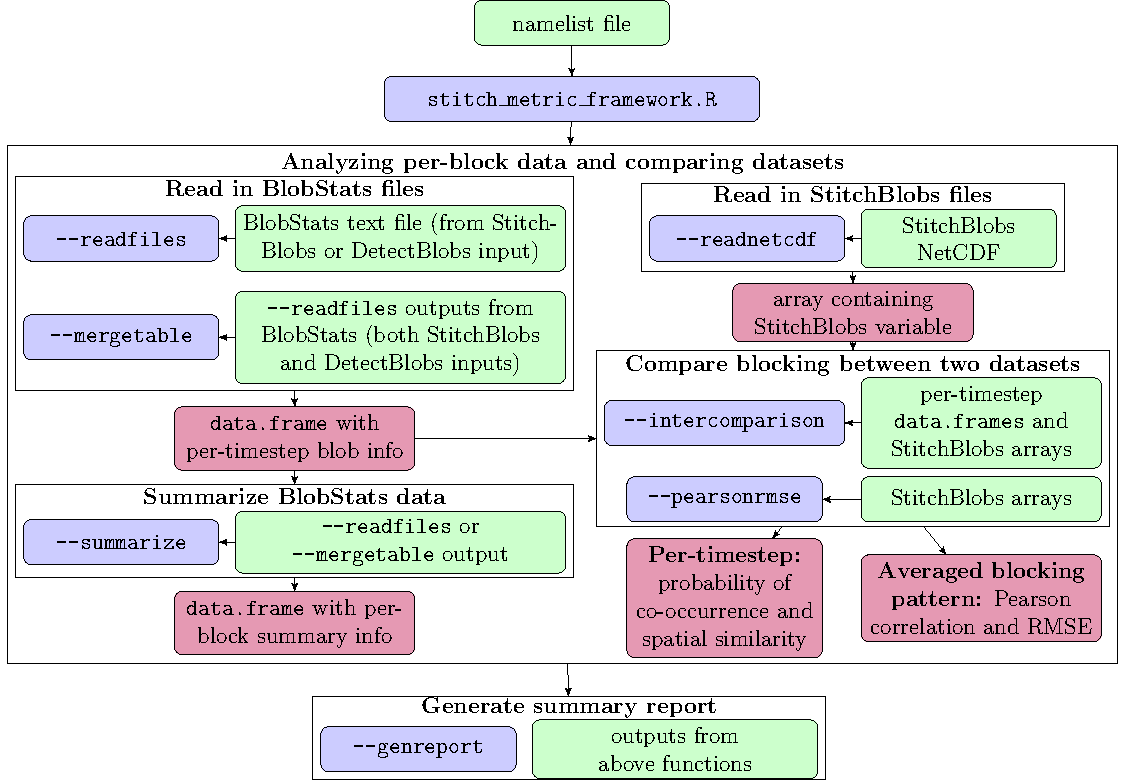
\includegraphics[width=\textwidth]{Framework_figure.pdf}
\caption{BlobMetrics schematic. Inputs are in green, analysis tools are in purple, and outputs are in pink.}\label{fig:schematic}
\end{figure}

\subsection{Read BlobStats files into a single table (\texttt{--readfiles})}\label{readfiles}
This utility takes each BlobStats file and reads the information into a single combined data frame. The columns of the data frame depend upon the included variables in the BlobStats output. Possible variables include \texttt{minlat, minlon, maxlat, maxlon, centlat, centlon,} and \texttt{area} and are specified when running BlobStats. By default, the outputs are saved in RData format, but there is optional functionality to save this output to text or CSV as well.

\subsubsection{Requirements}
Text files containing output from BlobStats. The format of these files is explained in more detail in Appendix \ref{blobformat}.

\subsubsection{Command line syntax}
\begin{verbatim}
Rscript --vanilla stitch_metric_framework.R [-rf] [-nl or -nlrf FILE]
\end{verbatim}

The following flags are required:
\begin{itemize}
\item[] \texttt{-rf} (\texttt{--readfiles}) \\ Tell program to read in BlobStats data
\item[]\texttt{-nl} (\texttt{--namelist}) or \texttt{-nlrf} (\texttt{--namelistrf}) \texttt{FILE}\\ Name of namelist file
\end{itemize}

%\subsubsection{Required namelist variables}
%\begin{itemize}
%\item[] \texttt{nrun\_rf}\\ Number of times to run \texttt{--readfiles}
%\item[] \texttt{nhrs}\\Number of hours per time step in data files (i.e. 6 is 6 hourly)
%\item[] \texttt{filename\_stitchblobs} or \texttt{filelist\_stitchblobs}\\ Single file containing BlobStats data or a text file containing a list of file names. Please use one or the other--- set the unused variable to a blank string (\texttt{""})
%\item[] \texttt{rfn\_stitch, txt\_stitch, csv\_stitch}\\ Optional output file names in RData, text, or CSV format (store the respective variable as a blank string to suppress output for that particular file format)
%\item[] \texttt{df\_stitchname}\\Optional variable name for the output data frame in the RData file. Defaults to \texttt{df\_tot} if string is left blank.
%\end{itemize}
%
%\subsection{Function syntax}
%
%To load and use  this function in an interactive R session, do
%\begin{verbatim}
%source("readfiles.R")
%desired_name<-read_stats_to_table(flist,nhrs,..)
%\end{verbatim}
%
%which will produce a \texttt{data.frame} object with the variable name \texttt{desired\_name}.
%
%The following arguments are required:
%\begin{itemize}
%\item[] \texttt{flist}\\ a vector object containing the BlobStats file names.
%\item[] \texttt{nhrs}\\ Time resolution in terms of hours (i.e. 6 for 6 hourly)
%\end{itemize}
%
%The following arguments are optional:
%\begin{itemize}
%\item[] \texttt{var}\\ Name of the objective blocking detection algorithm used to produce input files for StitchBlobs. If left blank, a column \texttt{var} will be filled with the string \texttt{VAR}
%\item[] \texttt{rfn, textfn, csvfn}\\Strings specifying output file names for RData, text, and CSV file formats. If left blank, the function will merely return the \texttt{data.frame} object to the console.
%\end{itemize}

\subsubsection{Output}\label{tableoutput}

An example output \texttt{data.frame} looks like this in the R console:
\begin{verbatim}
             datehour minlat maxlat minlon maxlon centlat centlon    area  area_km bnum var
1 1980-12-01 00:00:00     50     72    187    218    61.0   202.5 0.08299 42330251    1 TM90
2 1980-12-01 06:00:00     50     74    187    222    62.0   204.5 0.08980 45803790    1 TM90

                           file
1   ERA_1980_DJF_NP_Z_stats.txt
2   ERA_1980_DJF_NP_Z_stats.txt
\end{verbatim}

\begin{itemize}
\item[]\texttt{datehour}\\The date string in the format \texttt{YYYY-MM-DD HH:MM:SS}
\item[] \texttt{minlat, maxlat, minlon, maxlon, centlat, centlon}\\ Latitude and longitude coordinates for the block's extent and centroid
\item[] \texttt{area}\\ Fractional area of the block
\item[] \texttt{area\_km}\\area of the block in km$^2$
\item[] \texttt{var}\\ Algorithm name specified either by the \texttt{--algname} flag in the console or \texttt{var} in the function (default \texttt{VAR})
\item[] \texttt{bnum} \\The blob ID number as specified in the BlobStats file
\item[] \texttt{file} \\name of the BlobStats file which contains the specified blob information
\end{itemize}

%\section{Read previously created data table(s) into an R session}\label{combinetable}
%This utility reads output  generated in Section \ref{readfiles} into the R session and produces a single output \texttt{data.frame}. This function is particularly useful if attempting to examine data from multiple detection algorithms. There is optional functionality to save the output to one of three file types (RData, text, or CSV).
%
%\subsection{Requirements}
%Data tables produced using the procedure outlined in Section \ref{readfiles}. The tables can be in RData, text, or CSV file format.
%
%\subsection{Command line syntax}
%\begin{verbatim}
%Rscript --vanilla stitch_metric_framework.R [-rt] [-nl or -nlrt FILE] 
%\end{verbatim}
%
%The following flags are required:
%\begin{itemize}
%\item[] \texttt{-rt} (\texttt{--readtable}) \\ Tell program to read in BlobStats data
%\item[]\texttt{-nl} (\texttt{--namelist}) or \texttt{-nlrt} (\texttt{--namelistrt}) \texttt{FILE}\\ Name of namelist file
%\end{itemize}
%
%\subsubsection{Required namelist variables}
%
%\begin{itemize}
%\item[] \texttt{nrun\_rt}\\ Number of times to run \texttt{--readtable}
%\item[] \texttt{ftype\_rt}\\ Input file type (\texttt{"R"}, \texttt{"text"}, or \texttt{"CSV"})
%\item[] \texttt{filename\_read} or \texttt{filelist\_read}\\ Single file or list of files containing \texttt{--readfiles} output
%\item[] \texttt{rfn\_combine, txt\_combine, csv\_combine}\\Optional output file names in RData, text, or CSV format (store the respective variable as a blank string to suppress output for that particular file format)
%\item[] \texttt{df\_combinename}\\Optional variable name for the output data frame in the RData file. Defaults to \texttt{df\_data} if string is left blank.
%\end{itemize}
%\subsection{Function syntax}
%To load this function in an interactive R session, do
%\begin{verbatim}
%source("readtable.R")
%desired_name<-combine_dfs(flist,ftype,...)
%\end{verbatim}
%
%which will combine the loaded \texttt{data.frame} objects from each file into a single \texttt{data.frame} object with the variable name \texttt{desired\_name}.
%
%The following arguments are required:
%\begin{itemize}
%\item[] \texttt{flist}\\ a vector object containing the BlobStats file names.
%\item[] \texttt{ftype}\\ File format of input files (specify one of three strings: \texttt{"R"}, \texttt{"text"}, or \texttt{"CSV"})
%\end{itemize}
%
%The following arguments are optional:
%\begin{itemize}
%\item[] \texttt{rfn, textfn, csvfn}\\Strings specifying output file names for RData, text, and CSV file formats. If left blank, the function will merely return the \texttt{data.frame} object to the console.
%\end{itemize}
%
%\subsection{Output}
%The output is identical to that seen in Section \ref{tableoutput}, but there might be multiple values for the \texttt{var} column if combining tables with data from different algorithms.

\subsection{Handling instances of merging/splitting blobs (\texttt{--mergetable)}}\label{mergesection}
There are some instances where multiple blobs will merge into a single blob at a later date, or a single blob will split off into multiple blobs (this was noted in Sinclair 1995). This can cause BlobStats to produce latitude/longitude blob extents which are much larger than those of each individual blob, and the centroid coordinate will subsequently ``jump'' a noticeable distance from one time step to the next. 

The DetectBlobs binary in TempestExtremes  will produce output that is very similar to StitchBlobs output, but provides latitude/longitude extents for each unique feature; blobs which split off from larger features have their own separate identifier.


For example, here is output from StitchBlobs for one blob over 24 hours:
\begin{verbatim}
           datehour minlat maxlat minlon maxlon centlat centlon    area  area_km var bnum
1980-12-01 00:00:00     50     72    187    218    61.0   202.5 0.08299 42330251   Z    1
1980-12-01 06:00:00     50     74    187    222    62.0   204.5 0.08980 45803790   Z    1
1980-12-01 12:00:00     45     75    139    226    60.0   182.5 0.12303 62753232   Z    1
1980-12-01 18:00:00     43     75    138    231    59.0   184.5 0.13999 71403925   Z    1
\end{verbatim}

Here  is corresponding output from DetectBlobs:

\begin{verbatim}
           datehour minlat maxlat minlon maxlon centlat centlon    area  area_km var bnum
1980-12-01 00:00:00     50     72    187    218    61.0   202.5 0.08299 42330251   Z    1
1980-12-01 06:00:00     50     74    187    222    62.0   204.5 0.08980 45803790   Z    2
1980-12-01 12:00:00     50     75    187    226    62.5   206.5 0.09634 49139611   Z    3
1980-12-01 12:00:00     45     55    139    155    50.0   147.0 0.02670 13618721   Z    4
1980-12-01 18:00:00     49     75    186    231    62.0   208.5 0.10133 51684833   Z    5
1980-12-01 18:00:00     43     57    138    157    50.0   147.5 0.03866 19719092   Z    6
\end{verbatim}

Note that at times 12Z and 18Z, the detected blob in the StitchBlobs dataset (\texttt{bnum 1}) is actually comprised of two  blobs, because the smaller blob (\texttt{bnum 4} and \texttt{6} in the DetectBlobs dataset) is separate from the larger blob (\texttt{3} and \texttt{5} in the DetectBlobs output) at these time steps, but the smaller blob merges into the larger blob at a later time.

%\begin{verbatim}
%           datehour minlat maxlat minlon maxlon centlat centlon    area   area_km var bnum bnum2
%1980-12-01 00:00:00     50     72    187    218    61.0   202.5 0.08299  42330251   Z    1     1
%1980-12-01 06:00:00     50     74    187    222    62.0   204.5 0.08980  45803790   Z    1     1
%1980-12-01 12:00:00     45     55    139    155    50.0   147.0 0.02670  13618721   Z    1     4
%1980-12-01 12:00:00     50     75    187    226    62.5   206.5 0.09634  49139611   Z    1     3
%1980-12-01 18:00:00     43     57    138    157    50.0   147.5 0.03866  19719092   Z    1     6
%1980-12-01 18:00:00     49     75    186    231    62.0   208.5 0.10133  51684833   Z    1     5
%...
%1980-12-04 18:00:00     50     62    188    215    56.0   201.5 0.04389  22386730   Z    1    30
%1980-12-04 18:00:00     38     69    137    181    53.5   159.0 0.13772  70246079   Z    1    29
%1980-12-05 00:00:00     38     70    138    215    54.0   176.5 0.19310  98493450   Z    1     1
%1980-12-05 06:00:00     38     70    138    216    54.0   177.0 0.20088 102461751   Z    1     1
%\end{verbatim}

While these merged blobs only made up a small subset of instances in our own dataset, we recognize that this data might skew results with respect to distribution of block size or centroid coordinate. The \texttt{--mergetable} utility provides the option to distinguish between the individual blobs within the larger detected region. The summarization utility (Section \ref{summarysection}), which provides information on each unique block's size, speed, etc will note any instances in which there is blob merging. The user can then choose to keep or omit blobs in which there was merging. As with \texttt{--readfiles}, the output defaults to RData format but has optional text and CSV outputs as well.

\subsubsection{Requirements}
Separate files or file lists for StitchBlobs and DetectBlobs data. %If using the interactive R session, two separate data tables must first be produced using the method outlined in Section \ref{readfiles} or Section \ref{combinetable}). 

\subsubsection{Command line syntax}
\begin{verbatim}
Rscript --vanilla stitch_metric_framework.R [-mt] [-nl or -nlmt FILE]
\end{verbatim}

The following flags are required:
\begin{itemize}
\item[] \texttt{-mt} (\texttt{--mergetable}) \\ Tell program to merge the data from StitchBlobs and DetectBlobs
\item[]\texttt{-nl} (\texttt{--namelist}) or \texttt{-nlmt} (\texttt{--namelistmt}) \texttt{FILE}\\ Name of namelist file
\end{itemize}

%\subsubsection{Required namelist variables}
%
%\begin{itemize}
%\item[]\texttt{nrun\_mt}\\ Number of times to run \texttt{--mergetable}
%\item[] \texttt{ftype\_mt}\\ Input file type (\texttt{"R"}, \texttt{"text"}, or \texttt{"CSV"})
%\item[] \texttt{stitch\_file} or \texttt{stitch\_list}\\ Single file or list of files containing  data from StitchBlobs (generated using either \texttt{--readfiles} or \texttt{--readtable})
%\item[] \texttt{detect\_file} or \texttt{detct\_list}\\ Single file or list of files containing  data from DetectBlobs (generated using either \texttt{--readfiles} or \texttt{--readtable})
%\item[] \texttt{rfn\_merged, txt\_merged, csv\_merged}\\Optional output file names in RData, text, or CSV format (store the respective variable as a blank string to suppress output for that particular file format)
%\item[] \texttt{df\_merged}\\Optional variable name for the output data frame in the RData file. Defaults to \texttt{df\_merged} if string is left blank.
%\end{itemize}
%\subsection{Function syntax}
%
%
%To load this function in an interactive R session, do
%\begin{verbatim}
%source("mergetable.R")
%desired_name<-merge_dfs(df_stitch,df_nostitch,...)
%\end{verbatim}
%
%which will produce a \texttt{data.frame} object with the variable name \texttt{desired\_name}. Note that \texttt{df\_stitch} and \texttt{df\_nostitch} will need to be created using either \texttt{read\_table} or \texttt{combine\_tables}.
%
%The following arguments are required:
%\begin{itemize}
%\item[] \texttt{df\_stitch}\\ a data frame (created using \texttt{read\_table} or \texttt{combine\_tables}) containing BlobStats output with StitchBlobs data
%\item[] \texttt{df\_nostitch}\\ a data frame (created using \texttt{read\_table} or \texttt{combine\_tables}) containing BlobStats output with DetectBlobs data
%\end{itemize}
%
%The following arguments are optional:
%\begin{itemize}
%\item[] \texttt{rfn, textfn, csvfn}\\Strings specifying output file names for RData, text, and CSV file formats. If left blank, the function will merely return the \texttt{data.frame} object to the console.
%\end{itemize}

\subsubsection{Output}

The output \texttt{data.frame} looks similar to one returned by the first two methods, with the exception of an additional \texttt{bnum2} variable. When \texttt{bnum=bnum2}, the latitude/longitude extent is encompassing a single blob.

\begin{verbatim}
           datehour minlat maxlat minlon maxlon centlat centlon    area   area_km var bnum bnum2
1980-03-06 00:00:00     34     42    191    206    38.0   198.5 0.02822  14394019   Z    1     1
\end{verbatim}

When the two do not match, there are multiple blobs contained within the latitude/longitude extent of the original StitchBlobs output.

\begin{verbatim}
           datehour minlat maxlat minlon maxlon centlat centlon    area   area_km var bnum bnum2
1980-03-08 18:00:00     39     45    136    156    42.0   146.0 0.02500  12751612   Z    1    13
1980-03-08 18:00:00     32     51    194    222    41.5   208.0 0.07581  38667988   Z    1    12
\end{verbatim}

\subsection{Create a per-blob summary table (\texttt{--summarize})}\label{summarysection}
This utility reads in a data frame with per-timestep information and creates a table that provides per-blob information on quantities such a the blob's starting and ending centroid coordinates, the blob's duration in days, and others described in more detail below. %If desired, blobs which are comprised of multiple blobs that merge into a single blob are omitted.

\subsubsection{Requirements}

RData containing output from \texttt{--readfiles} or \texttt{--mergetable}.

\subsubsection{Command line syntax}

\begin{verbatim}
Rscript --vanilla stitch_metric_framework.R [-st] [-nl or -nlst FILE]
\end{verbatim}

The following flags are required:
\begin{itemize}
\item[] \texttt{-st} (\texttt{--summarize})\\ Tell program to summarize each unique blob's data
\item[]\texttt{-nl} (\texttt{--namelist}) or \texttt{-nlst} (\texttt{--namelistst}) \texttt{FILE}\\ Name of namelist file
\end{itemize}

%\subsubsection{Required namelist variables}
%\begin{itemize}
%\item[]\texttt{nrun\_st}\\ Number of times to run \texttt{--summarize}
%\item[] \texttt{ftype\_st}\\ Input file type (\texttt{"R"}, \texttt{"text"}, or \texttt{"CSV"})
%\item[] \texttt{filename\_summ} or \texttt{filelist\_summ}\\ Single file or list of files containing  data from StitchBlobs (generated using either \texttt{--readfiles} or \texttt{--readtable})
%\item[] \texttt{keep\_merge}\\ Keep or omit blobs which are comprised of multiple blobs? If \texttt{TRUE}, all blobs are kept; if \texttt{FALSE}, blobs where the \texttt{merged} column has a value of \texttt{YES} are omitted from the output.
%\item[] \texttt{rfn\_summ, txt\_summ, csv\_summ}\\Optional output file names in RData, text, or CSV format (store the respective variable as a blank string to suppress output for that particular file format)
%\item[] \texttt{df\_summ}\\Optional variable name for the output data frame in the RData file. Defaults to \texttt{df\_summ} if string is left blank.
%\end{itemize}

%\subsection{Function syntax}
%To load this function in an interactive R session, do
%\begin{verbatim}
%source("summarize.R")
%desired_name<-gen_summary_table(df_in,...)
%\end{verbatim}
%
%which will summarize each unique blob in the input \texttt{data.frame} object and produce an output \texttt{data.frame} object with the variable name \texttt{desired\_name}. Note that \texttt{df\_in} will need to be created using either \texttt{read\_table} or \texttt{combine\_tables}.
%
%The following arguments are required:
%\begin{itemize}
%\item[] \texttt{df\_in}\\ Name of the input data frame (create using methods from Section \ref{readfiles} or \ref{combinetable}).
%\end{itemize}
%
%The following arguments are optional:
%\begin{itemize}
%\item[] \texttt{keep\_merge} \\ Default is \texttt{TRUE}; if set to \texttt{FALSE}, the final data table will not contain merged blobs.
%\item[] \texttt{rfn, textfn, csvfn}\\Strings specifying output file names for RData, text, and CSV file formats. If left blank, the function will merely return the \texttt{data.frame} object to the console.
%\end{itemize}

\subsubsection{Output}
An example summary table looks like this in the R console:
\begin{verbatim}
             startdate             enddate duration_days merged start_centlat
1  1980-03-06 00:00:00 1980-03-14 12:00:00          8.50    YES          38.0
2  1980-03-17 06:00:00 1980-03-26 00:00:00          8.75     NO          39.5

   start_centlon end_centlat end_centlon   dist_km zonal_dist_km
1          198.5        43.5       194.0  719.2533      379.0267
2          204.0        39.0       208.5  391.4136      387.4485

   zonal_speed_kph min_area  max_area avg_area var bnum
1        1.8579740 12751612  75295717 32349835   Z    1
2        1.8449929 15500859  35505588 32349835   Z    2
\end{verbatim}

\begin{itemize}
\item[]\texttt{startdate, enddate}\\The date string in the format \texttt{YYYY-MM-DD HH:MM:SS}
\item[] \texttt{duration\_days}\\ Number of days that block persists
\item[] \texttt{merged}\\ Checks whether or not the block extent is the result of multiple blobs merging (see Section \ref{mergesection}). If this value is \texttt{YES}, then it is recommended to check the per-timestep information in order to see when and where the blobs merge, as well as how it affects the calculation of the block size and centroid.
\item[] \texttt{start\_centlat, start\_centlon, end\_centlat, end\_centlon}\\ start and end coordinates of block centroid.
\item[] \texttt{dist\_km}\\ Great circle distance from start to end coordinates.
\item[] \texttt{zonal\_dist\_km} \\ Only the zonal component of the distance between the start and end coordinates (calculated using the start and end longitude coordinates of the centroid and the midpoint of the start and end latitude coordinates).
\item[] \texttt{zonal\_speed\_kph} \\Average speed, in km/hr, of the block's movement. Calculated as distance over duration.
\item[] \texttt{min\_area, max\_area, avg\_area} \\ Various information for the block size, in km$^2$
\item[] \texttt{var}\\Algorithm name (as provided previously when reading in the BlobStats data)
\item[] \texttt{bnum}\\ The block ID number from BlobStats (might differ from the ID number of DetectBlobs output)
\end{itemize}


\subsection{Reading in NetCDF data (\texttt{--readnetcdf})}

This utility reads data from NetCDF files into arrays in R, combining data from multiple files if desired. There is an optional utility to read in only a geographical subset of the data, as well as the ability to save the specified variables to either a single NetCDF output file or an Rdata file.

\subsubsection{Requirements}
NetCDF files with the desired variables. Note that if reading multiple files into a single session, they should all contain the variables that are specified in the command line or function call, otherwise the utility will throw an exception. 

If the dataset is very large, it might cause R to crash due to memory constraints (although this is dependent upon the available system memory--- this scenario is more likely to happen on personal computers). It is recommended to split the data up by time or regional subsets if this is likely to be a problem.

\subsubsection{Command line syntax}

\begin{verbatim}
Rscript --vanilla stitch_metric_framework.R [-rn] [-nl or -nlrn FILE]
\end{verbatim}

The following flags are required:

\begin{itemize}
\item[] \texttt{-rn (--readnetcdf)}\\Tell program to read NetCDF data into R.
\item[]\texttt{-nl} (\texttt{--namelist}) or \texttt{-nlrn} (\texttt{--namelistrn}) \texttt{FILE}\\ Name of namelist file
\end{itemize}

%\subsubsection{Required namelist variables}
%\begin{itemize}
%\item[] \texttt{nrun\_rn}\\ Number of times to run \texttt{--readnetcdf}
%\item[] \texttt{filename\_netcdf} or \texttt{filelist\_netcdf} Single NetCDF file name or list of NetCDF file names
%\item[] \texttt{varvec}\\ Vector of variable names to be read to R in the format \texttt{c("VAR1","VAR2","VAR3"...)}
%\item[] \texttt{outvec}\\ Vector of output variable names (must be same length as \texttt{varvec}
%\item[] \texttt{outrdata, outnetcdf}\\ Optional output file names in RData or NetCDF format
%\item[] \texttt{timename}\\Name of time axis
%\item[] \texttt{levname}\\Name of vertical axis
%\item[] \texttt{latname}\\Name of latitude axis
%\item[] \texttt{lonname} \\Name of longitude axis
%\item[] \texttt{minlat, maxlat, minlon, maxlon} \\ subsetting boundaries for horizontal (lat/lon) direction; if not subsetting, set variable to blank string (\texttt{""})
%\item[] \texttt{minlev,maxlev}\\ If applicable, subsetting boundaries for the vertical axis. If subsetting to a single level (i.e. 500 mb) set both \texttt{minlev} and \texttt{maxlev} to that value. If vertical axis doesn't exist, set variable to blank string (\texttt{""})
%\end{itemize}
%
%\subsection{Function syntax}
%
%To load this function in an interactive R session, do\begin{verbatim}
%source("read_netCDF_to_R.R")
%vlist<-c("VAR1","VAR2","VAR3")
%vars_output<-read_netcdf(flist,vlist,...)
%\end{verbatim}
%
%The folllowing arguments are required:
%\begin{itemize}
%\item[] \texttt{flist}\\ Vector containing input NetCDF file names
%\item[] \texttt{vlist}\\Vector containing variable names that will be read into R
%\end{itemize}
%
%which will read all of the NetCDF variables into R matrices and return a \texttt{list} object with the name \texttt{vars\_output} containing all of the resulting output variables, as well as the axes for time, latitude, longitude, etc. 
%
%The following arguments are optional:
%\begin{itemize}
%\item[] \texttt{olist}\\ Vector containing variable names of output variables (default is the input variable list)
%\item[] \texttt{timename, levname, latname, lonname}\\ Names of the axis variables (defaults are \texttt{"time", "lev", "lat", "lon"})
%\item[] \texttt{minlat, maxlat, minlon, maxlon, minlev, maxlev}\\ Coordinates of lat/lon extent and vertical levels, if subsetting. 
%\item[]\texttt{ncout, rdataout}\\ Strings specifying output file names for NetCDF and RData file formats. If left blank, the function will return a \texttt{list} object that contains all of the variables. 
%\end{itemize}



\subsubsection{Output}

%If neither \texttt{ncout} nor \texttt{rdataout} are specified, the function returns a \texttt{list} object (here named \texttt{vars\_output} as per the example).
%
%Each variable stored within \texttt{vars\_output} can be accessed via \texttt{vars\_output[["VAR"]]}. In order to turn the \texttt{vars\_output} object into distinct R variables that are accessible from the global environment, do the following:
%
%\begin{verbatim}
%list_variables<-names(vars_output)
%for (v in list_variables){
%    assign(v,vars_output[[v]])
%}
%remove(vars_output)
%\end{verbatim}
%\texttt{list\_variables} is a vector of names of all of the variables that are contained within \texttt{vars\_output}. This sequence of commands will store each variable in \texttt{vars\_output} in the global environment, then delete the \texttt{list} object (for space saving purposes).
%\subsubsection{NetCDF}
%The returned NetCDF will contain the variables specified by the user, with axes \texttt{time\_axis, lat\_axis, lon\_axis} and, optionally, \texttt{lev\_axis} (not all variables are on multiple vertical levels). Currently, the output NetCDF does not contain the metadata from the original file, although this might change in the future.
%
%\texttt{time\_axis} is in units of \texttt{hours since 1800-01-01 00:00} regardless of the original time units. 

%\subsubsection{RData}

The RData file contains the axis variables (\texttt{time\_axis, lev\_axis, lat\_axis, lon\_axis}), a vector of string date times (\texttt{time\_format}), and the variables specified within the variable list. 

\subsection{Comparing two datasets on a per-timestep basis (\texttt{--intercomparison})}

This utility  provides information about the amount of agreement between the two datasets with respect to detected blocks. This agreement is quantified by the following metrics:
\begin{itemize}
%\item \textbf{ Pearson pattern correlation:} Strength of linear relationship between blocking frequency values at corresponding coordinates for the two datasets. Note: there will be high correlation when the \textit{pattern} is similar, regardless of the relative magnitudes.
%\item \textbf{Root mean square error (RMSE):} Measure of differences in blocking frequency values between the two datasets.
\item \textbf{Probability of co-occurrence:} The likelihood that a block will appear at a location in dataset 1  given that it also appears at a similar location in dataset 2.
\item \textbf{Spatial similarity:} When a block is present, amount of field that is commonly designated as blocked by both datasets. 
\end{itemize}

\subsubsection{Requirements}

Per-timestep blob information (from either \texttt{--readfiles} or \texttt{--mergetable}) and the corresponding arrays from \texttt{--readnetcdf}. Both files should be in RData format.

\subsubsection{Command line syntax}
\begin{verbatim}
Rscript --vanilla stitch_metric_framework.R [-ic] [-nl or -nlrn FILE]
\end{verbatim}


The following flags are required:

\begin{itemize}
\item[] \texttt{-ic (--intercomparison)}\\Tell program to compare the two datasets specified in the namelist.
\item[]\texttt{-nl} (\texttt{--namelist}) or \texttt{-nlic} (\texttt{--namelistic}) \texttt{FILE}\\ Name of namelist file
\end{itemize}

\subsubsection{Output}

The RData file contains the following variables:
\begin{itemize}
\item \texttt{df\_analyze}: The input data from both datasets (similar to output seen in Section \ref{readfiles} or \ref{mergesection}), combined into a single \texttt{data.frame}
\item \texttt{df\_overlaps}: A \texttt{data.frame} variable that lists all instances where a blob from dataset 1 overlaps with a blob from dataset 2. An example output, where \texttt{V1} denotes the ERA-Interim reanalysis and \texttt{V2} denotes the JRA reanalysis, would look like this:
\begin{verbatim}
                datehour similarity V1bnum V1bnum2 V1minlat V1maxlat V1minlon V1maxlon
6829 2005-02-25 18:00:00  0.8806536      5       5       31       42      162      190
6830 2005-02-26 00:00:00  0.8718225      5       5       30       41      163      191
6831 2005-02-26 06:00:00  0.8957676      5       5       30       41      166      191
6832 2005-02-26 12:00:00  0.8561735      5       5       30       41      168      191
6833 2005-02-26 18:00:00  0.8239728      5       5       31       41      170      191
6834 2005-02-27 00:00:00  0.7644073      5       5       31       40      173      191

     V1centlat V1centlon V2bnum V2bnum2 V2minlat V2maxlat V2minlon V2maxlon V2centlat
6829      36.5     176.0      5       5    31.25    41.25   162.50   190.00    36.250
6830      35.5     177.0      5       5    31.25    41.25   163.75   190.00    36.250
6831      35.5     178.5      5       5    31.25    41.25   166.25   191.25    36.250
6832      35.5     179.5      5       5    31.25    41.25   168.75   191.25    36.250
6833      36.0     180.5      5       5    31.25    40.00   171.25   190.00    35.625
6834      35.5     182.0      5       5    32.50    40.00   173.75   190.00    36.250

     V2centlon
6829   176.250
6830   176.875
6831   178.750
6832   180.000
6833   180.625
6834   181.875
\end{verbatim}
\item \texttt{p1given2} and \texttt{p2given1}: probability of co-occurrence for dataset 1 given dataset 2 and the reverse.
\item \texttt{sim\_25}, \texttt{sim\_50} and \texttt{sim\_75}: the 25th, 50th, and 75th percentile values of spatial similarity between the two datasets.
\item \texttt{V1} and \texttt{V2}: The names of your variables for dataset 1 and dataset 2.
\end{itemize}

\subsection{Comparing the average blocking frequency of two datasets (\texttt{pearsonrmse})}
This utility quantifies the agreement between two blocking frequency patterns. Note that the two datasets need to have the same grid spacing for this utility to work.

\subsubsection{Requirements}

Arrays from \texttt{--readnetcdf} in RData format.

\subsubsection{Command line syntax}

\begin{verbatim}
Rscript --vanilla stitch_metric_framework.R [-pr] [-nl or -nlpr FILE]
\end{verbatim}

The following flags are required:

\begin{itemize}
\item[] \texttt{-pr (--pearsonrmse)}\\Tell program to compare the two datasets specified in the namelist.
\item[]\texttt{-nl} (\texttt{--namelist}) or \texttt{-nlpr} (\texttt{--namelistpr}) \texttt{FILE}\\ Name of namelist file
\end{itemize}

\subsubsection{Output}


\subsection{Create a summary report (\texttt{--genreport})}

This utility takes the inputs from previous sections and creates a summary report with information 
\pagebreak

\begin{appendix}
\section{BlobStats File Format}\label{blobformat}
Each BlobStats file is formatted as follows:\begin{itemize}
\item[] Line 1: Tab-separated column names 
\item[]Blob information line: \texttt{Blob IDNUM (NUM\_TIMESTEPS)} where \texttt{IDNUM} is the blob's unique identifier number and \texttt{NUM\_TIMESTEPS} is the number of timesteps in the blob's lifespan.
\item[] Per-timestep blob information: Always contains the timestep number in column 1. The other columns depend on the included variables. 
\end{itemize}

For example, a BlobStats file with two Blobs, each with a lifetime of 2 time steps, would look like this:

\begin{verbatim}
time,minlat,maxlat,minlon,maxlon,centlat,centlon,area
Blob 1 (2)
1992-03-13-43200        33.00000        43.00000        130.00000       142.00000       38.00000        136.00000       0.02783
1992-03-13-64800        33.00000        43.00000        130.00000       144.00000       38.00000        137.00000       0.03289
Blob 2 (2)
1992-03-24-64800        28.00000        36.00000        132.00000       149.00000       32.00000        140.50000       0.03461
1992-03-25-00000        27.00000        37.00000        131.00000       151.00000       32.00000        141.00000       0.04569
\end{verbatim}



\end{appendix}


\end{document}
